\chapter{Problem Description}

\section{Available Data}
	{
		XXX field region Witzwil, Data from gregor perich (ref xxx)
		fields over 5 years 
		cereals (not other cultures)
	}
	\subsection{Yieldmapping Data}{
		XXX description of how harvester gets data, knn-interpolation and rsterization, reference to gregors paper
		\begin{figure}
			\centering
			\begin{subfigure}{.5\textwidth}
			  \centering
			  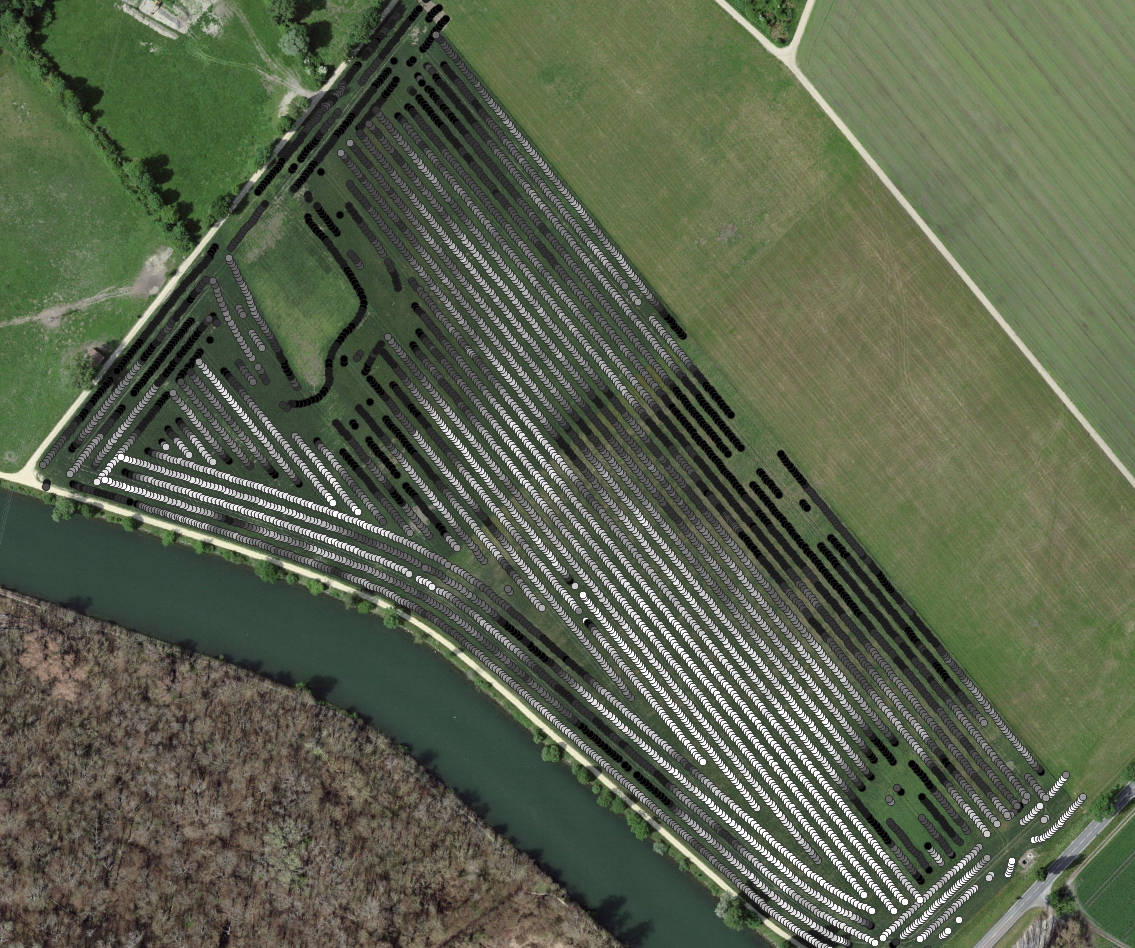
\includegraphics[height=.75\linewidth]{satelite/witzwil_2021_P112_yield_harvester_cropped.png}
			  \caption{A subfigure XXX}
			%   \label{fig:sub1}
		\end{subfigure}%
		\begin{subfigure}{.5\textwidth}
			\centering
			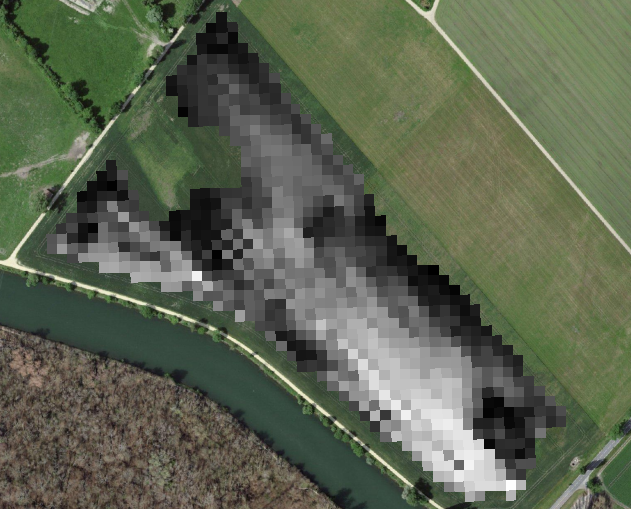
\includegraphics[height=.75\linewidth]{satelite/witzwil_2021_P112_yield_cropped.png}
			  \caption{A subfigure xxx}
			%   \label{fig:sub2}
			\end{subfigure}
			\caption{xxx}
			\label{fig:test}
		\end{figure}
	}

	\subsection{Sentinel 2 Satellite Image Data}{
		\subsubsection*{General Information}{
			DE:
			Die ESA \footnote{XXX reference: https://sentinel.esa.int/web/sentinel/missions/sentinel-2}
			revisit times = 5 days am Äquator
			mittlere breitengrade 2-3 tage
			XXX CH-grafik von LukasGraf?
			witzwil befindet

		}

		\subsubsection*{Data Description}{
			\begin{table}[h]
				\caption{XXX SCL classes}
				\label{tab:satelite/scl_classes}
				\center
				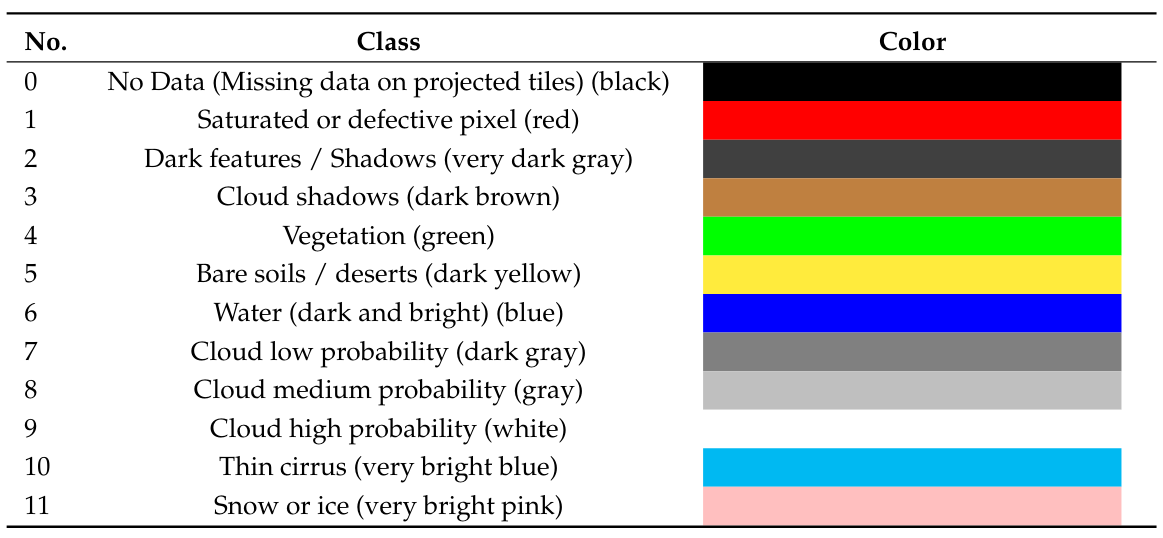
\includegraphics[width=0.8\textwidth]{satelite/scl_classes.png}
			\end{table}
			
			\begin{figure}[h]
				\label{fig:satelite/sentinel-2-bands}
				\center
				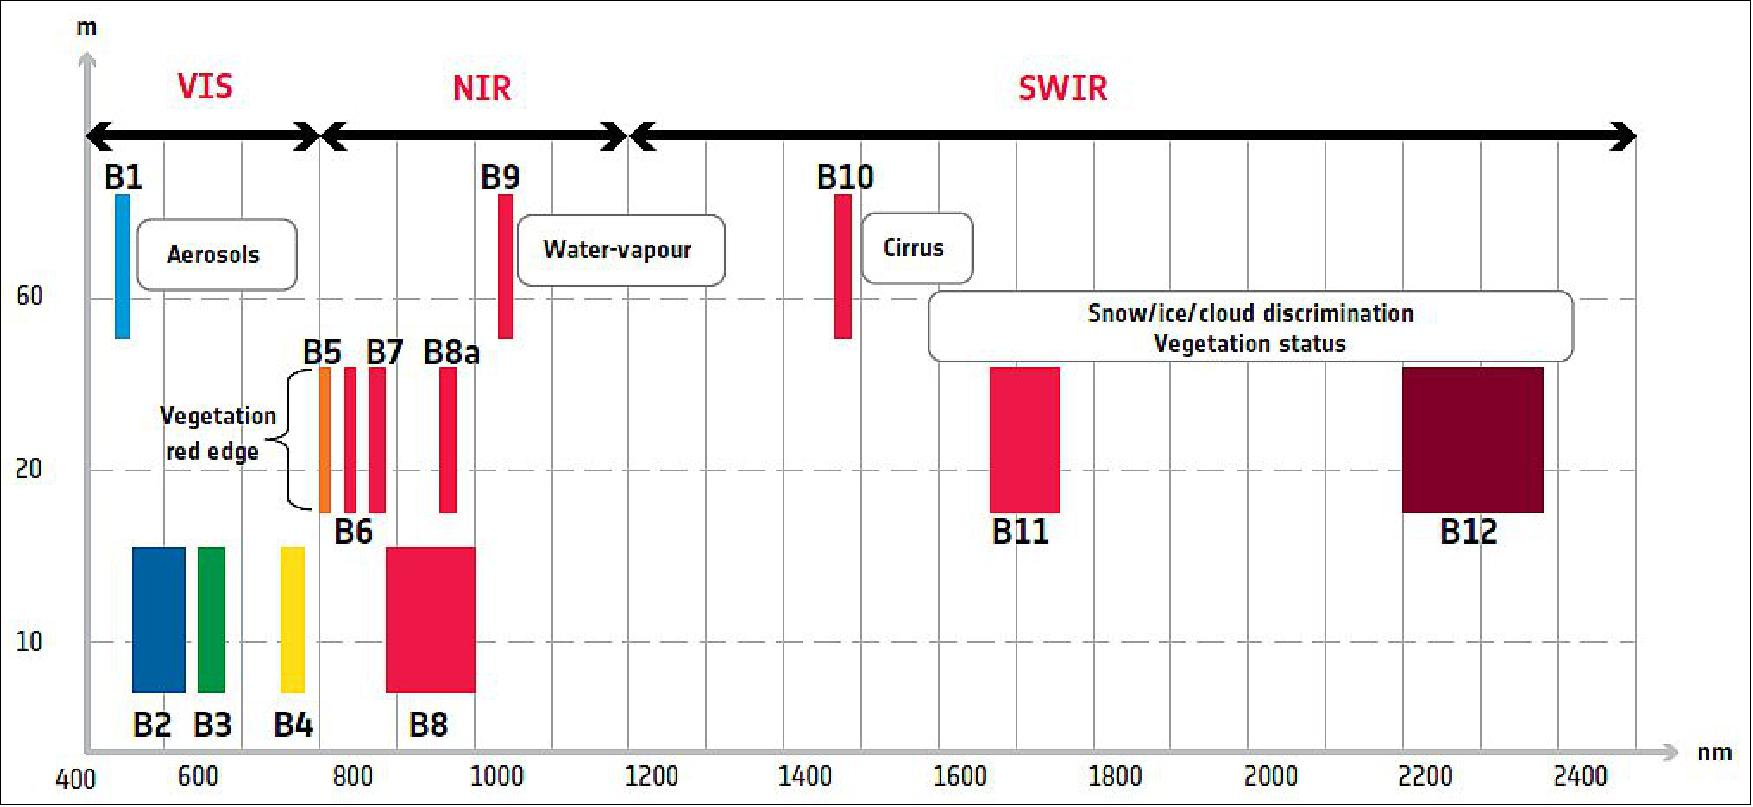
\includegraphics[width=0.4\textwidth]{satelite/sentinel-2-bands.jpg}
				\caption{XXX Sentinel 2 bands}
			\end{figure}
		}

		\subsubsection*{Data Illustration}{
			xxx plot beschreiben
			% 2x3 plot
				%satelite/time_series_2021_P112/15_scl5_2021-02-23.png
	%satelite/time_series_2021_P112/30_scl4_2021-05-09.png
	%satelite/time_series_2021_P112/33_scl9_2021-05-24.png
	%satelite/time_series_2021_P112/35_scl4_2021-06-03.png
	%satelite/time_series_2021_P112/40_scl10_2021-06-28.png
	%satelite/time_series_2021_P112/45_scl2_2021-07-23.png

\begin{figure*}
	\centering
	\begin{subfigure}[b]{0.31\textwidth}
		\centering
		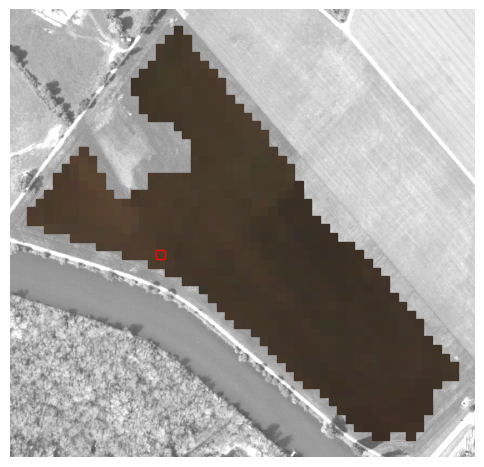
\includegraphics[width=\textwidth]{satelite/time_series_2021_P112/15_scl5_2021-02-23.png}
		\caption[2021-02-23\hspace*{0.1cm} SCL 5]%
		{{\small 2021-02-23\hspace*{0.1cm} SCL 5}}    
		\label{fig:satelite/time_series_2021_P112/15_scl5_2021-02-23.png}
	\end{subfigure}
	\hfill
	\begin{subfigure}[b]{0.31\textwidth}  
		\centering 
		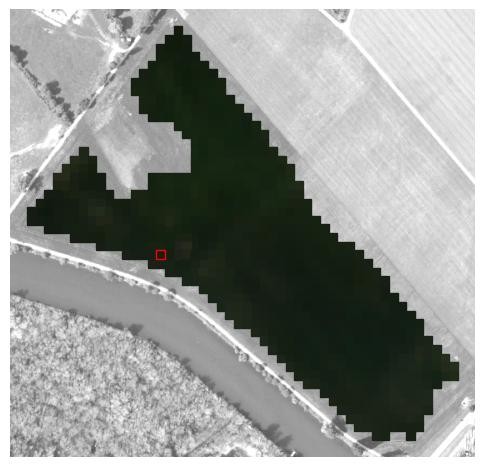
\includegraphics[width=\textwidth]{satelite/time_series_2021_P112/30_scl4_2021-05-09.png}
		\caption[2021-05-09\hspace*{0.1cm} SCL 4]%
		{{\small 2021-05-09\hspace*{0.1cm} SCL 4}}    
		\label{fig:satelite/time_series_2021_P112/30_scl4_2021-05-09.png}
	\end{subfigure}
	\hfill
	\begin{subfigure}[b]{0.31\textwidth}  
		\centering 
		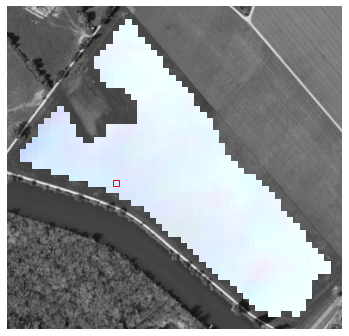
\includegraphics[width=\textwidth]{satelite/time_series_2021_P112/33_scl9_2021-05-24.png}
		\caption[2021-05-24\hspace*{0.1cm} SCL 9]%
		{{\small 2021-05-24\hspace*{0.1cm} SCL 9}}    
		\label{fig:satelite/time_series_2021_P112/33_scl9_2021-05-24.png}
	\end{subfigure}

	\vskip\baselineskip
	\begin{subfigure}[b]{0.31\textwidth}   
		\centering 
		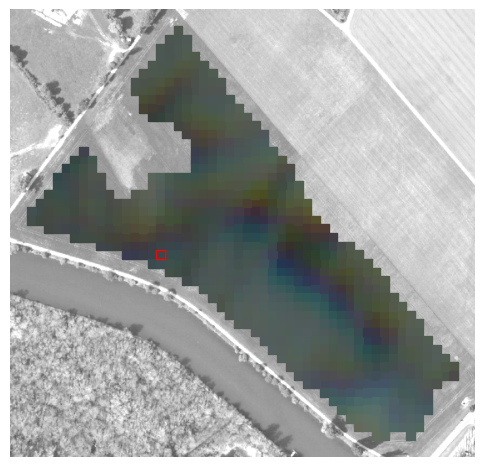
\includegraphics[width=\textwidth]{satelite/time_series_2021_P112/35_scl4_2021-06-03.png}
		\caption[2021-06-03\hspace*{0.1cm} SCL 4]%
		{{\small 2021-06-03\hspace*{0.1cm} SCL 4}}    
		\label{fig:satelite/time_series_2021_P112/35_scl4_2021-06-03.png}
	\end{subfigure}
	\hfill
	\begin{subfigure}[b]{0.31\textwidth}   
		\centering 
		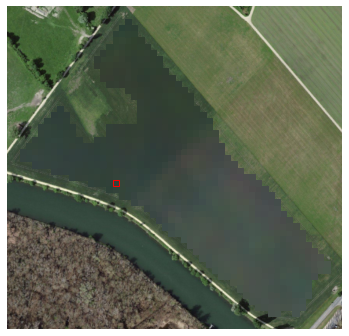
\includegraphics[width=\textwidth]{satelite/time_series_2021_P112/40_scl10_2021-06-28.png}
		\caption[2021-06-28\hspace*{0.1cm} SCL 10]%
		{\small 2021-06-28\hspace*{0.1cm} SCL 10}    
		\label{fig:satelite/time_series_2021_P112/40_scl10_2021-06-28.png}
	\end{subfigure}
	\hfill
	\begin{subfigure}[b]{0.31\textwidth}  
		\centering 
		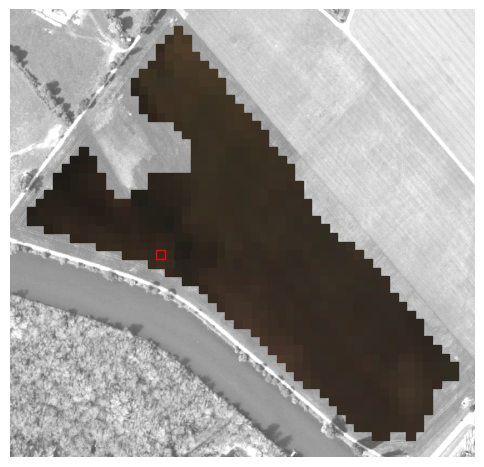
\includegraphics[width=\textwidth]{satelite/time_series_2021_P112/45_scl2_2021-07-23.png}
		\caption[2021-07-23\hspace*{0.1cm} SCL 2]%
		{{\small 2021-07-23\hspace*{0.1cm} SCL 2}}    
		\label{fig:satelite/time_series_2021_P112/45_scl2_2021-07-23.png}
	\end{subfigure}

	\vskip\baselineskip
	\begin{subfigure}[b]{0.7\textwidth}   
		\centering 
		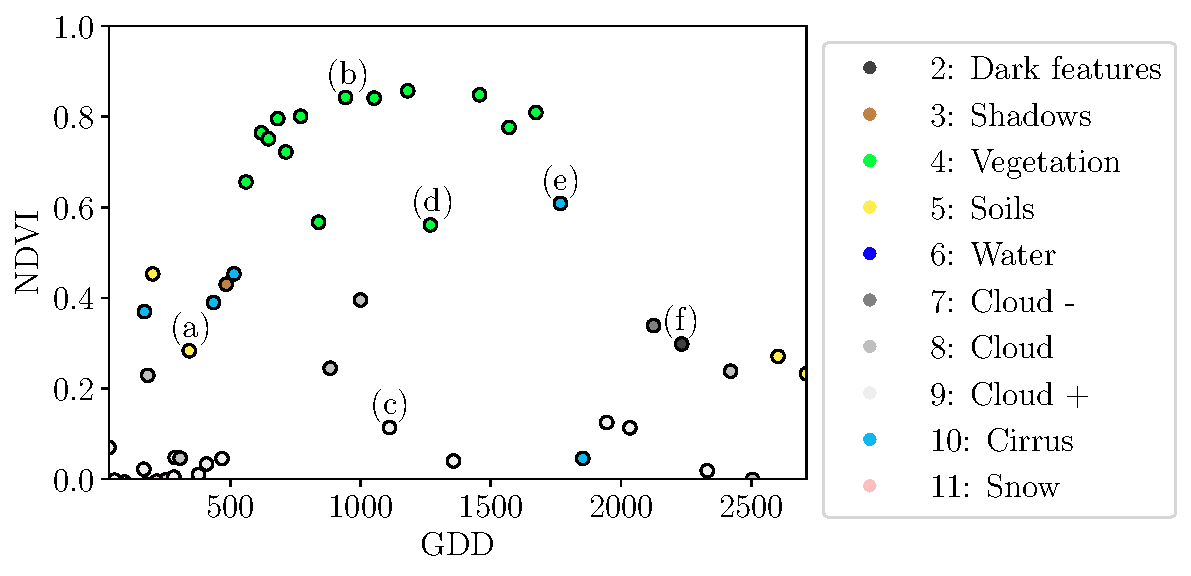
\includegraphics[width=\textwidth]{interpol/ndvi_ts_scl.pdf}
		\caption[Corresponding NDVI {TS}]%
		{{\small Corresponding NDVI {TS}}}    
		\label{fig:interpol/ndvi_ts_scl45_grey.pdf}
	\end{subfigure}
	\vspace{0.3cm}
	\caption[Satellite images of a field at selected times + NDVI TS]{Satellite images of a field at selected times with a static grayscale background for orientation. Moreover, the NDVI {TS} of the red-highlighted pixel is shown in (g) colored by the SCL labels.} 
	\label{fig:witzwil_selected_satellite_images}
\end{figure*}



			% Description of plot
			In fig.~\ref{fig:witzwil_selected_satellite_images} 

			DE:  
			Die Abb.~\ref{fig:witzwil_selected_satellite_images} zeigt eine Auswahl von 6 Satelitenbildern von einer Parzelle, welche unsere Herrausvorderungen aufzeigen. Im Februar (Bild(a)) sehen wir wie erwartet keine Vegetation, sondern nackte Erde. Anfang Mai beobachten wir ein wolkenfreies dunkelgrünes feld. In (c) wird ersichtlich, dass wir bei starker Bewölkung keine Hoffnung haben nützliche information zu erhalten. Bild (d) zeigt auf, dass die SCL-Klassifizierung nicht zuverlässig ist. In (e) sehen wir ein blasses Grün. Vermutlich sehen wir durch zirrus wolken hindurch.   
			
			%% subfigures references:
			% (see. \ref{fig:satelite/time_series_2021_P112/15_scl5_2021-02-23.png})
			% (see. \ref{fig:satelite/time_series_2021_P112/30_scl4_2021-05-09.png})
			% (see. \ref{fig:satelite/time_series_2021_P112/33_scl9_2021-05-24.png})
			% (see. \ref{fig:satelite/time_series_2021_P112/35_scl4_2021-06-03.png})
			% (see. \ref{fig:satelite/time_series_2021_P112/40_scl10_2021-06-28.png})
			% (see. \ref{fig:satelite/time_series_2021_P112/45_scl2_2021-07-23.png})
		}
	}






